\documentclass[justified]{tufte-handout}
\usepackage{braph2_tut}
%\geometry{showframe} % display margins for debugging page layout

\title{Prepare brain connectivity data}

\author[The BRAPH~2 Developers]{The BRAPH~2 Developers}

\begin{document}

\maketitle

\begin{abstract}
\noindent
This Tutorial explains how to prepare and work with brain connectivity data, where we have one connectivity matrix per subject such as in the case of diffusion weighted imaging tractography. 
\end{abstract}

\tableofcontents

\fig{figure*}
	{fig:01}
	{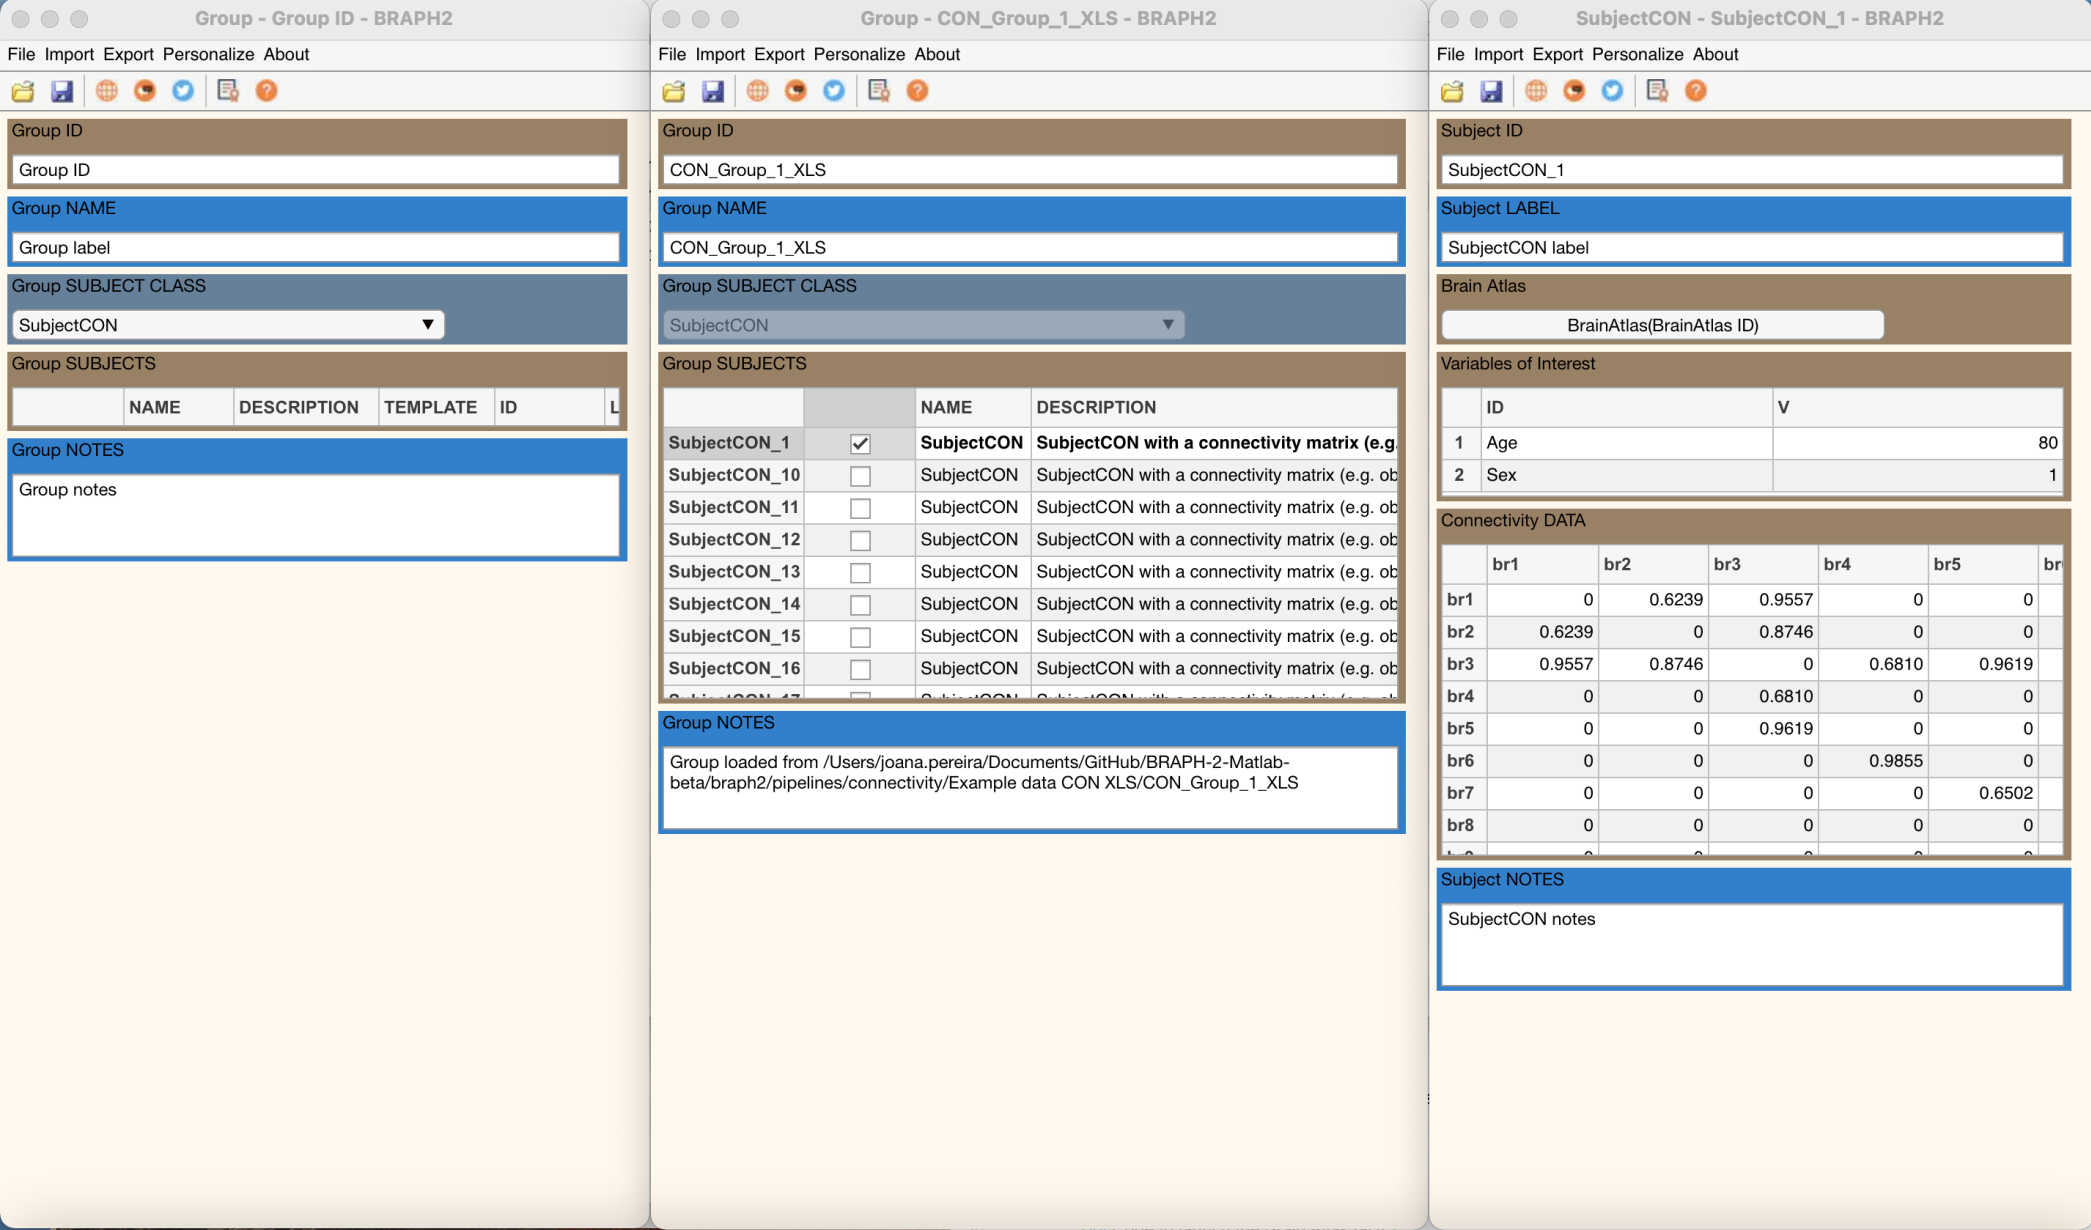
\includegraphics[height=10cm]{tut_gr_conn/fig01.png}}
	{Brain Connectivity Group GUI}
	{
	Full graphical user interface to work with brain connectivity group data in BRAPH~2.0. 
	}

\clearpage
\section{Open the GUI}

The group GUI is the second step after you have selected a brain atlas. You can open it by typing \code{braph2} in the MatLab's terminal, which allows you to select a pipeline containing the steps required to perform your analysis and upload a brain atlas. After these steps have been completed you can upload your group's data, as shown in \Figref{fig:02}a.

\fig{figure*}
	{fig:02}
	{
	[h!]
	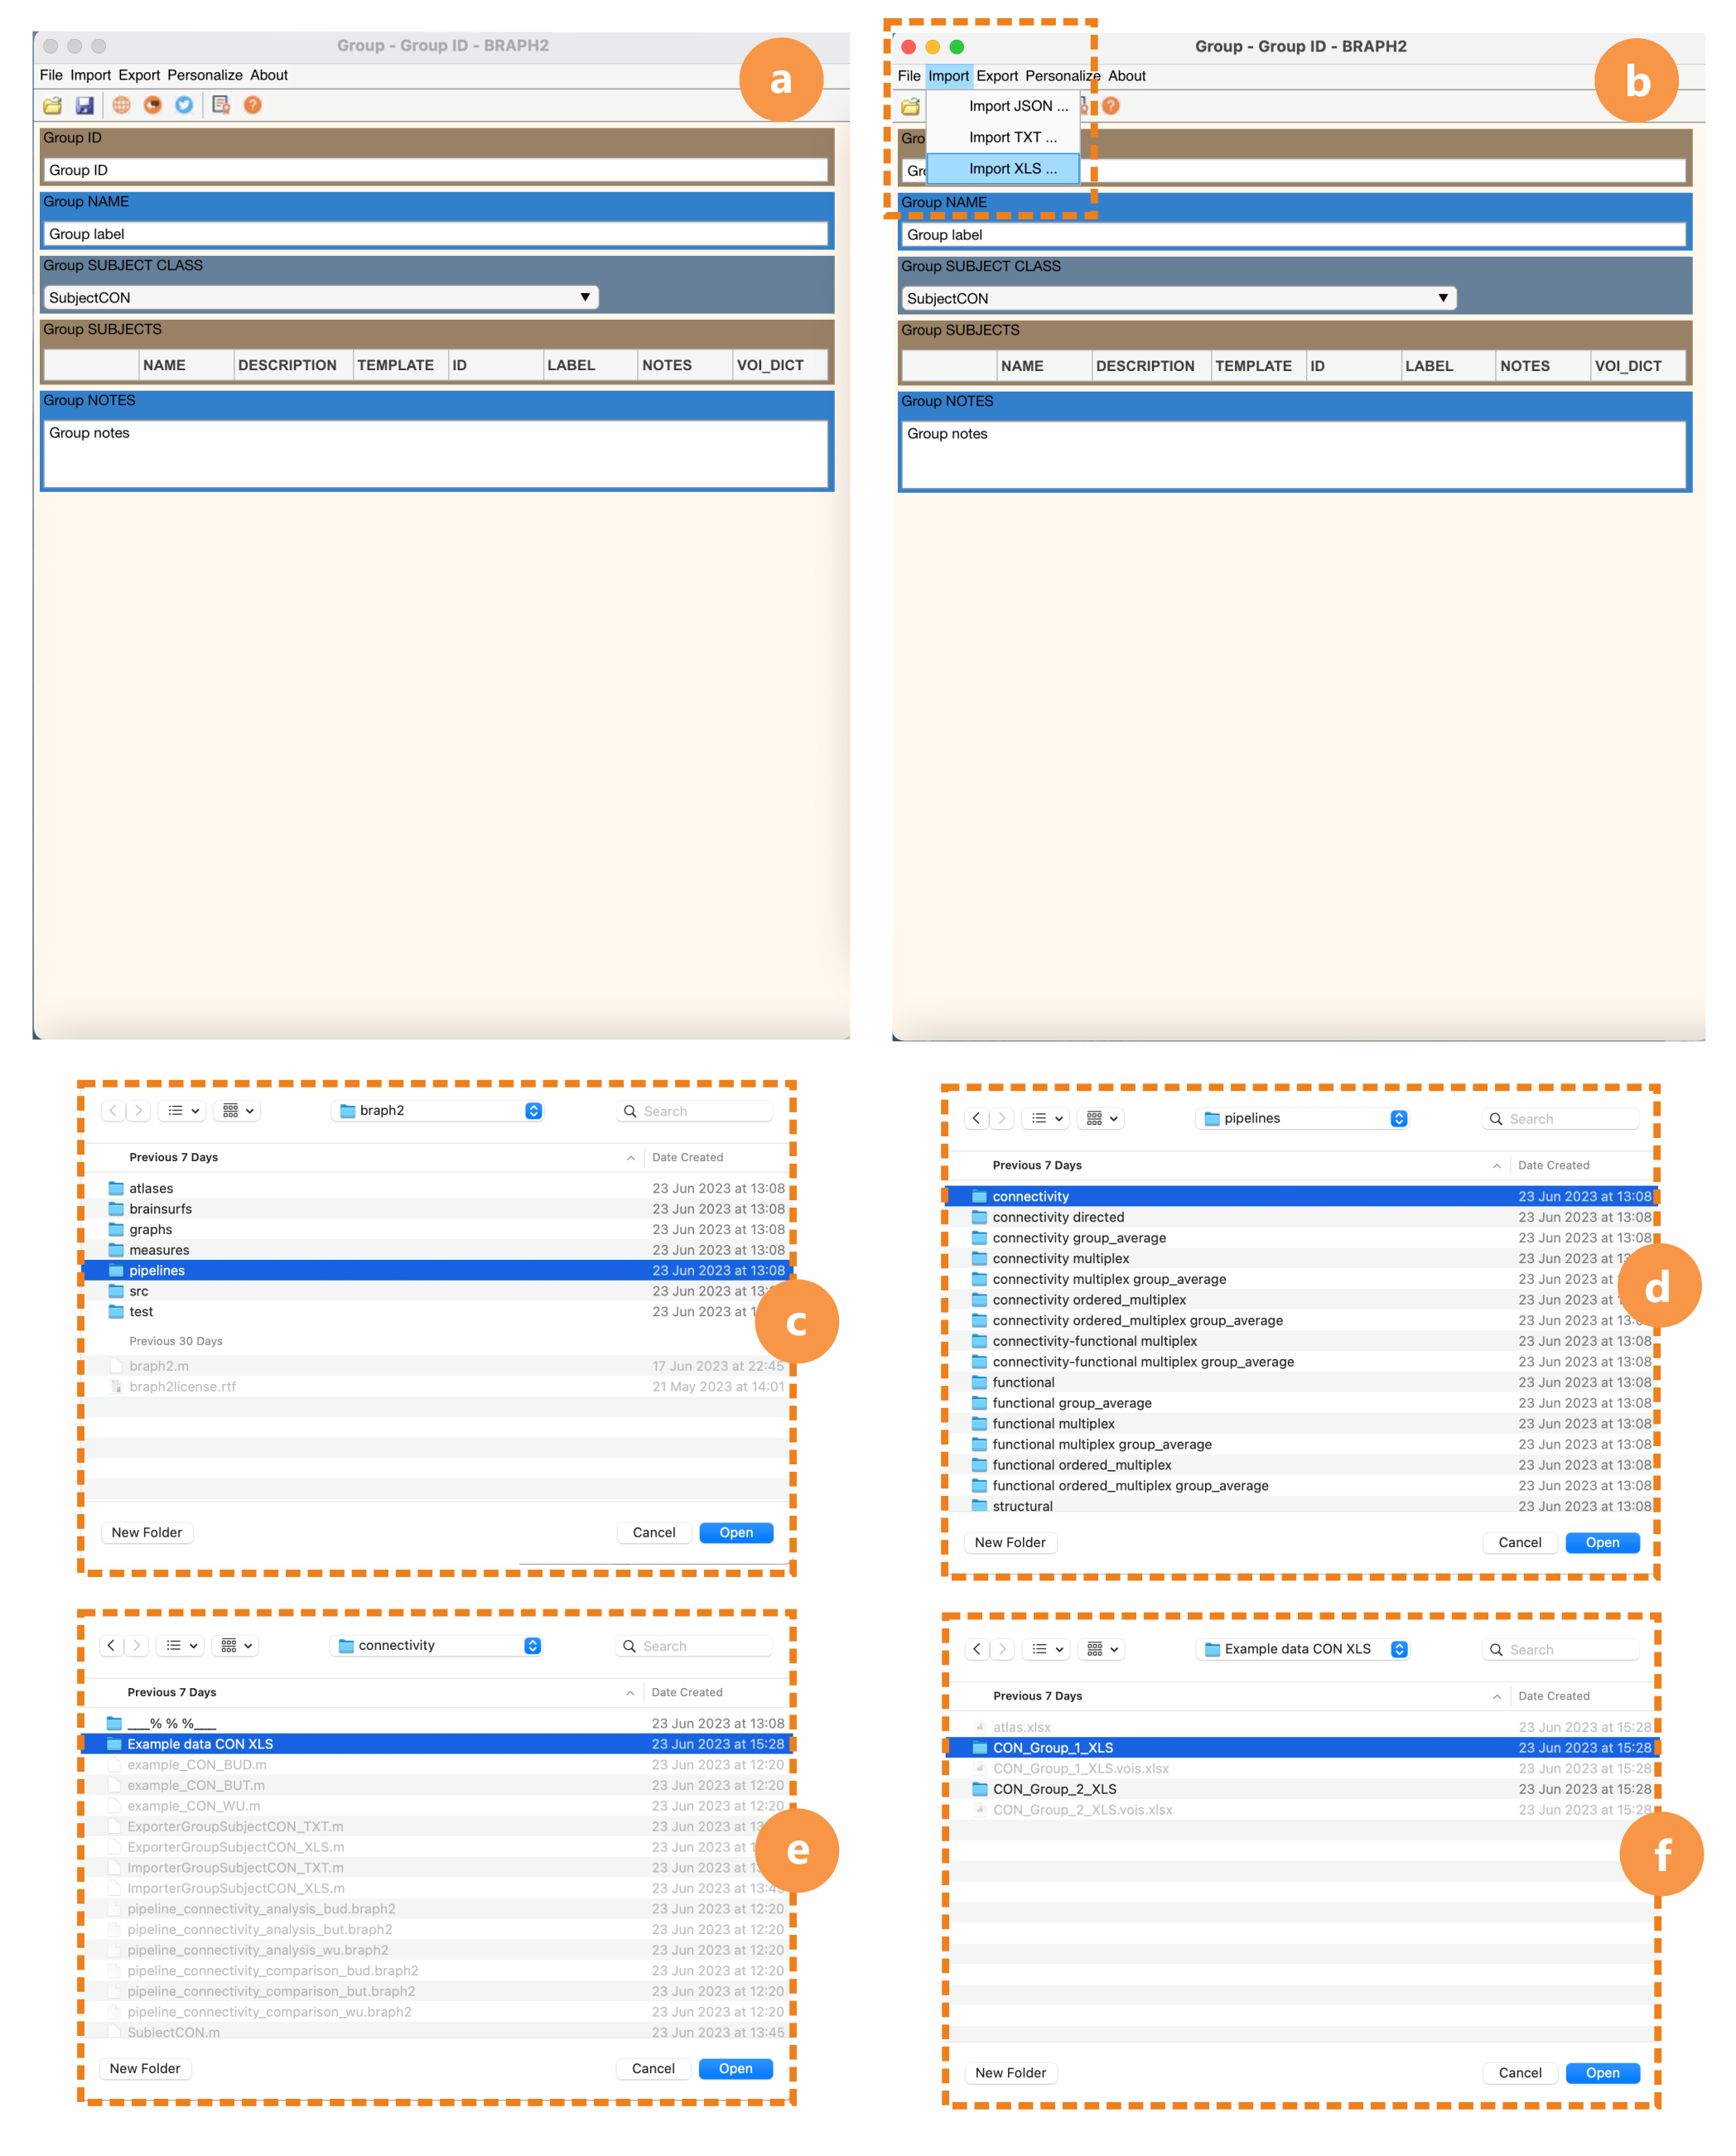
\includegraphics[height=10cm]{tut_gr_conn/fig02.png}
	}
	{Upload a brain atlas}
	{
	The different steps you need to follow to open brain connectivity data using the GUI: 
	{\bf a} Open the group GUI.
	{\bf b} Import a folder containing the connectivity matrices in XLS or TXT format.
	{\bf c} Navigate to the BRAPH~2.0 folder \fn{pipelines}.
	{\bf d} Navigate to the BRAPH~2.0 folder \fn{connectivity}.
	{\bf e} Navigate to the BRAPH~2.0 folder \fn{Example data CON XLS}.
	{\bf f} Select the folder containing the connectivity matrices of one group \fn{CON\_Group\_1\_XLS}.
	}

To open the GUI and upload the brain connectivity data, you can also do it from the command line (i.e., without opening an analysis pipeline) by typing the commands in \Coderef{cd:launch}.
%
\begin{lstlisting}[
	label=cd:launch,
	caption={
		{\bf Code to launch the Brain Connectivity Group GUI.}
		This code can be used in the MatLab command line to launch the Brain Connectivity Group without having to open a pipeline.
	}
]
gr = Group('SUB_CLASS', 'SubjectCON'); ¥\circled{1}\circlednote{1}{creates a new object \code{Group}.}¥

gui = GUIElement('PE', gr); ¥\circled{2}\circlednote{2}{creates a GUI to upload the group data.}¥
gui.get('DRAW')¥\circled{3}\circlednote{3}{draws the GUI.}¥
gui.get('SHOW') ¥\circled{4}\circlednote{4}{shows the GUI.}¥
\end{lstlisting}

\clearpage
\section{Visualize the Brain Connectivity Group data}

After launching the previous steps (\Figref{fig:02}) you can visualize the data (Figref{fig:03}a), change the Group ID, name and notes (Figref{fig:03}b). 

\fig{figure*}
	{fig:04}
	{
	[h!]
	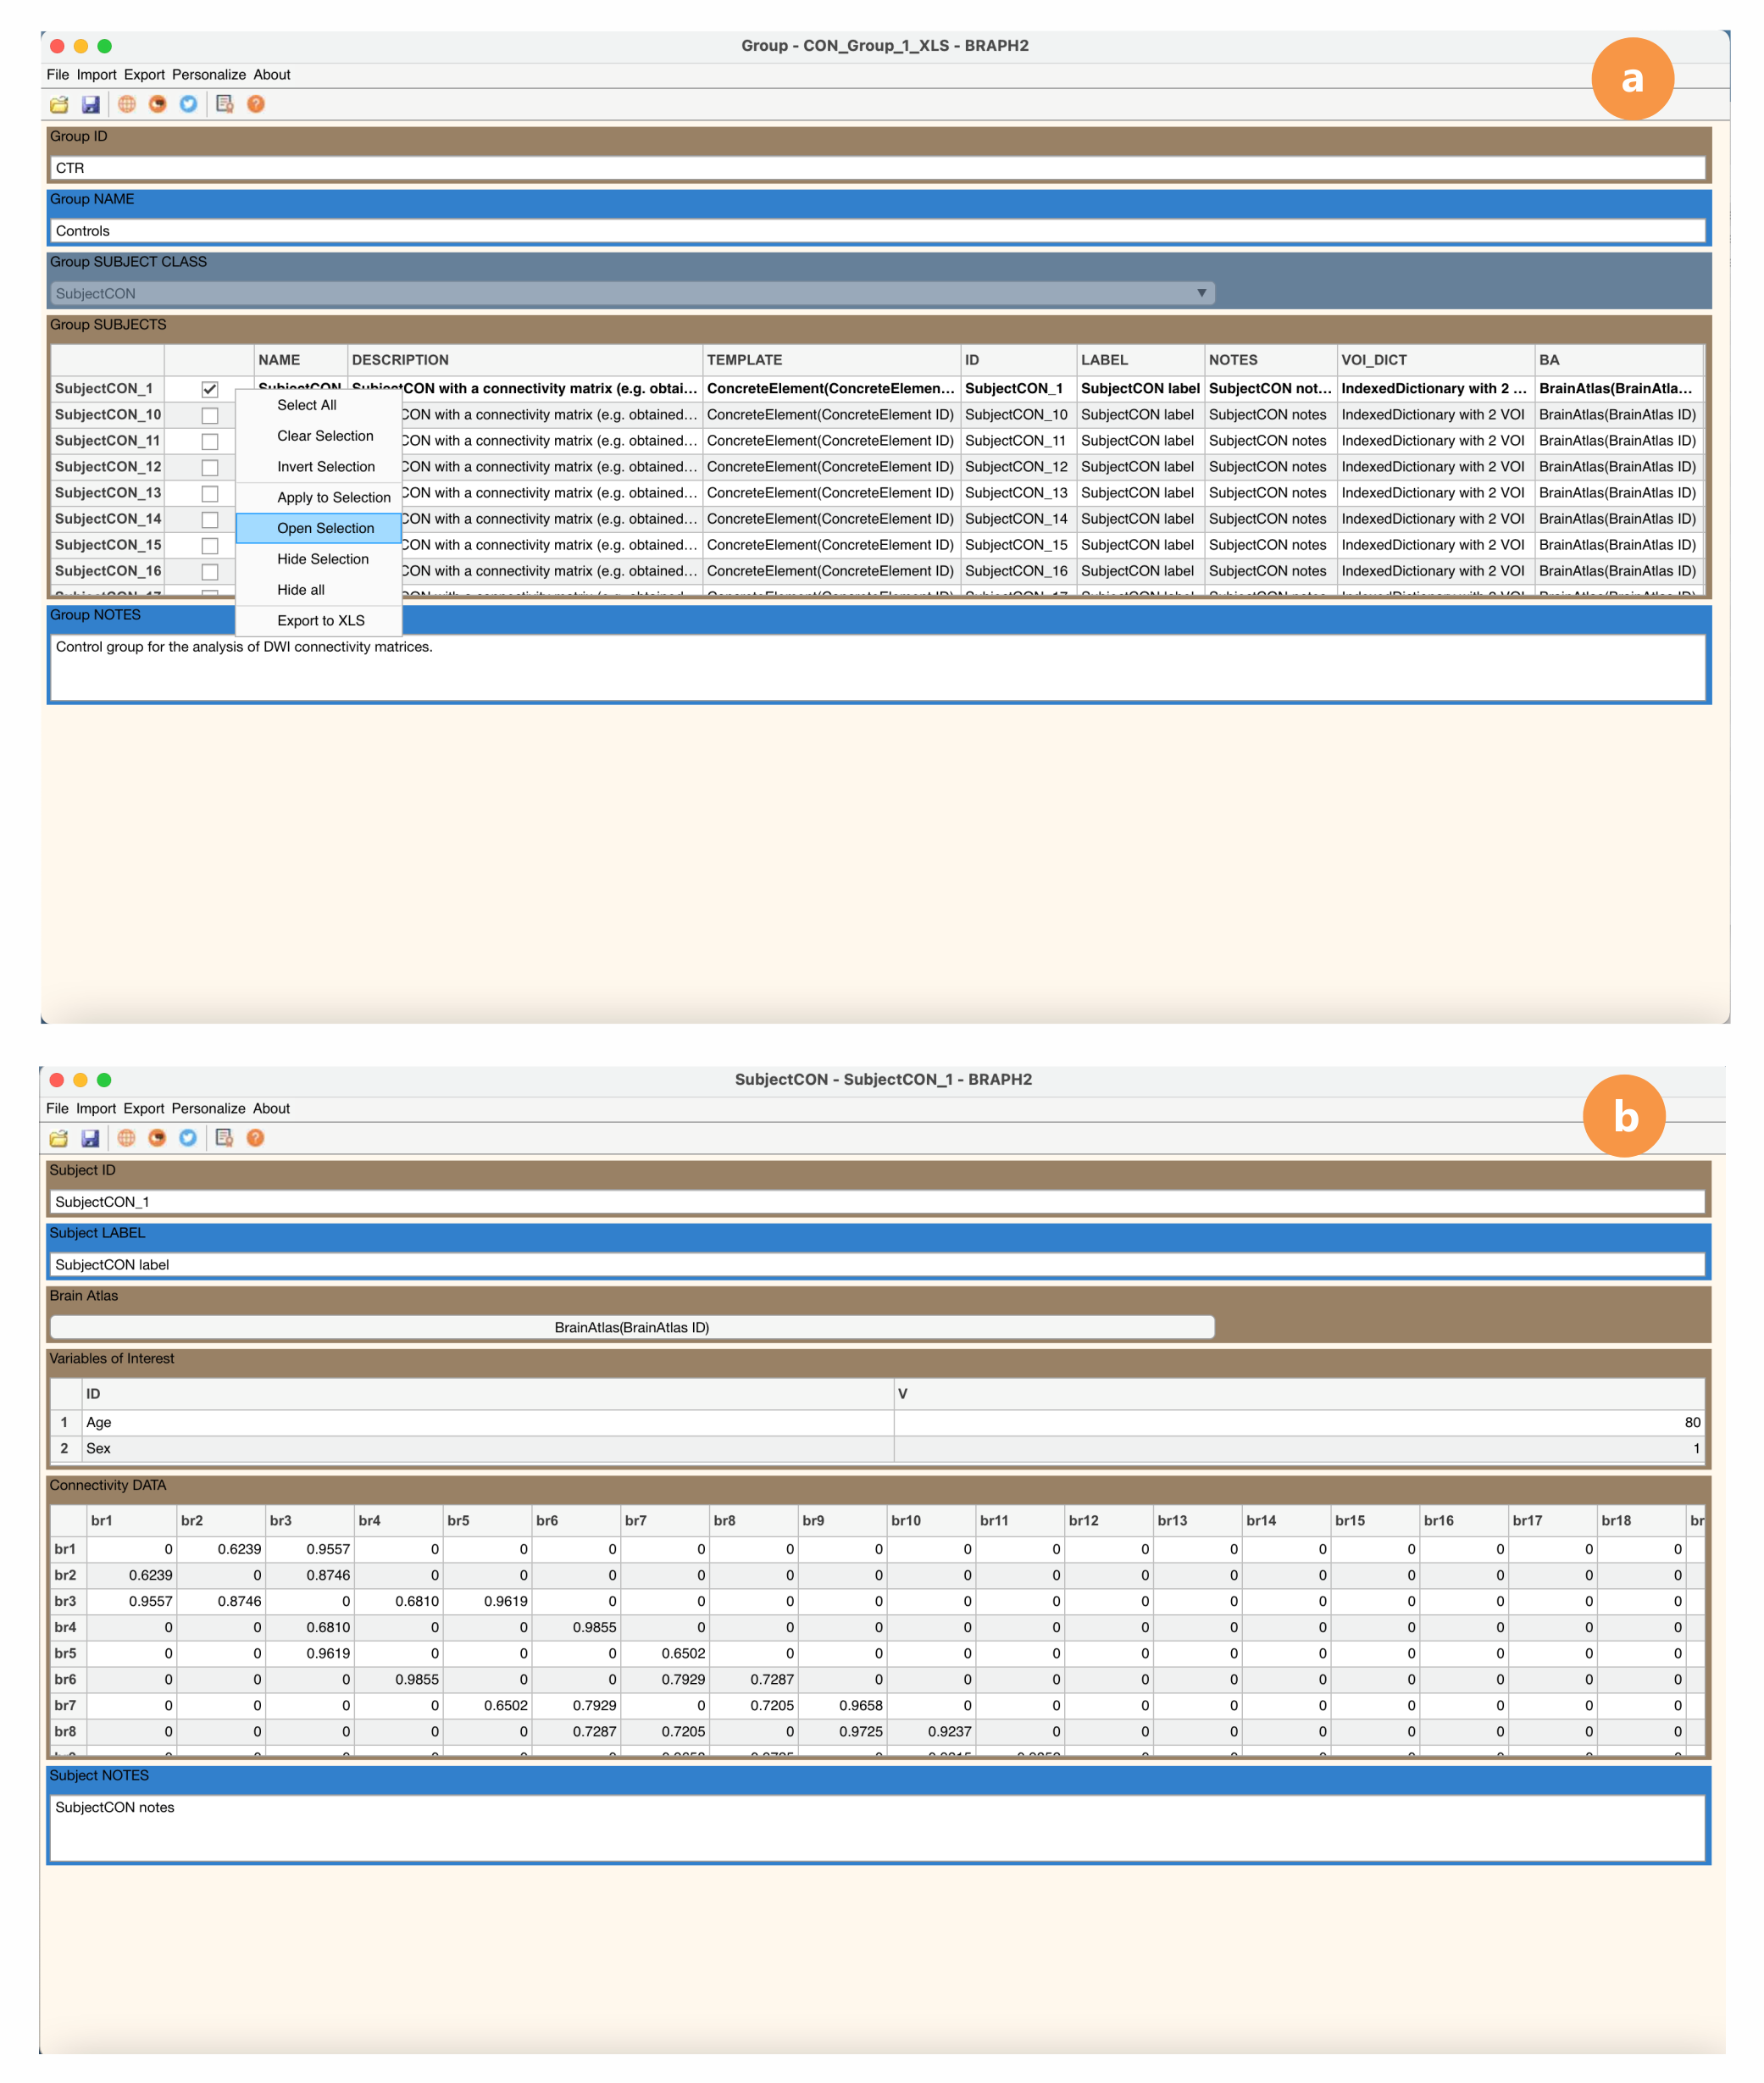
\includegraphics{tut_gr_conn/fig04.png}
	}
	{Edit the Brain Connectivity Group data}
	{
	Information that can be changed in the Brain Connectivity Group GUI: 
	{\bf a} The ID, name, and notes.
	{\bf b} The values of the connectivity matrix.
	}

Finally you can open a subject's connectivity matrix by selecting the subject, right click and select "Open selection" (Figref{fig:04}a), which will show the matrix values (Figref{fig:04}b). You can also change the ID, label, age, sex and even the values of your connectivity matrix.
	

\section{Adding covariates}

It is very common to have covariates in an analysis. In BRAPH~2.0, these covariates should be included in a separate excel file outside the group's folder, have the same name as the folder in addition to ".vois" as shown in \Figref{fig:05}a), where "vois" stand for variables of interest. This covariates file should have a specific format, where the first two rows have the following information:

\begin{itemize}

\item Covariates names (row 1, column 1). 
For example: Subject ID, Age and Sex. In this example we have added a new covariate: Education.

\item Covariates values (row 2, column 1). 
For example: Female and Male (Sex) or Low and High (Education).

\fig{figure*}
	{fig:05}
	{
	[h!]
	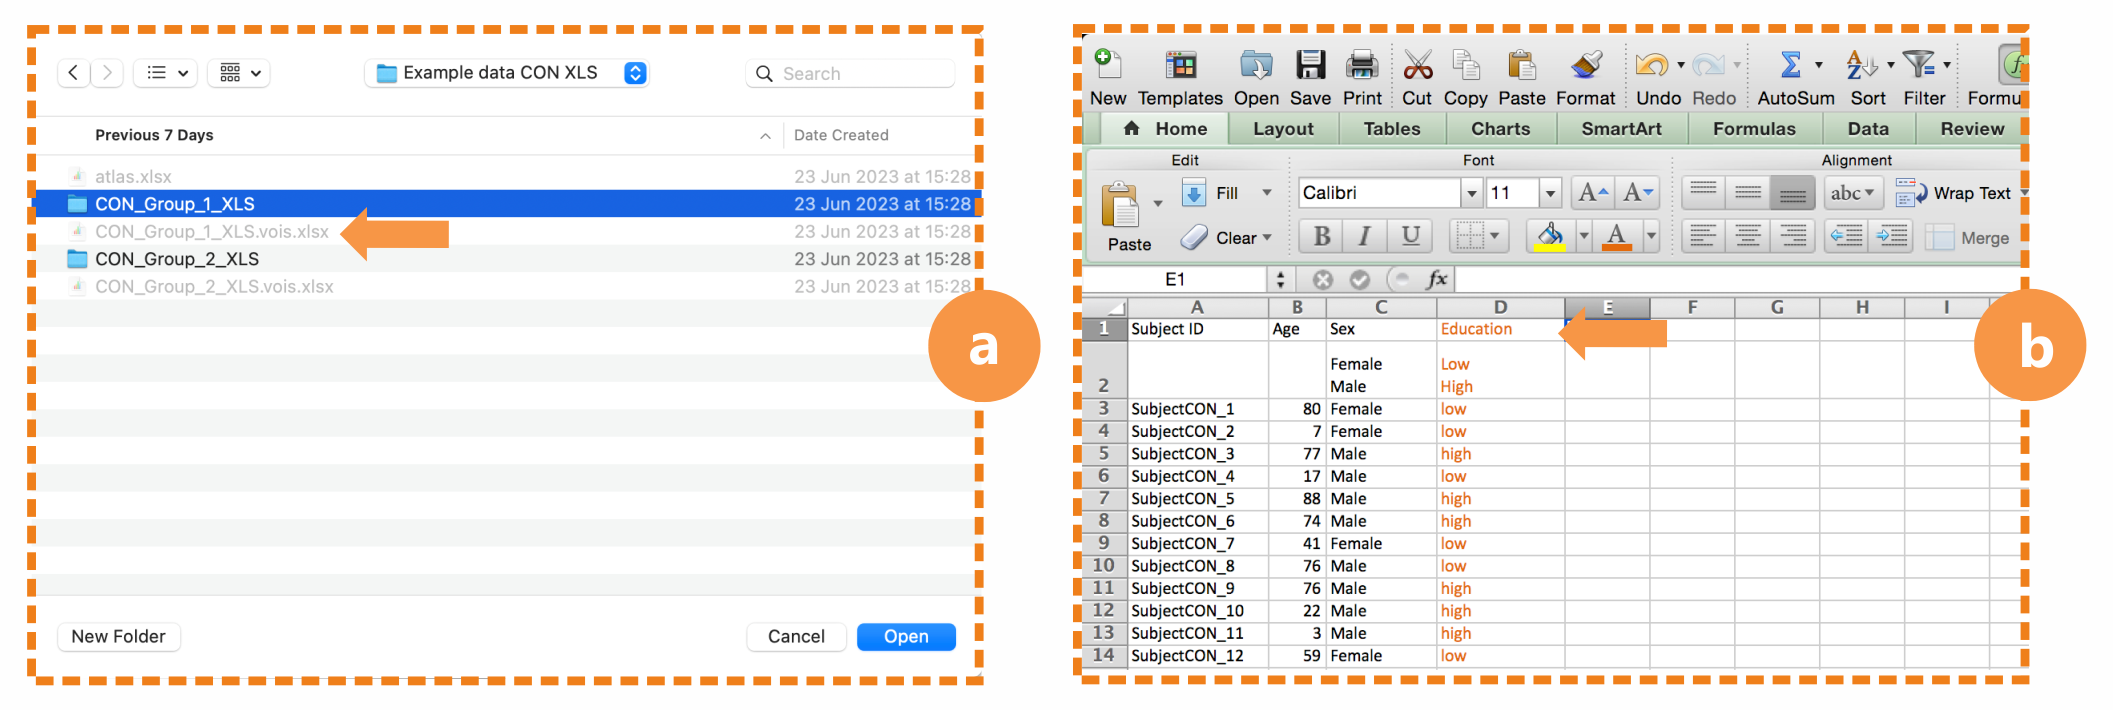
\includegraphics{tut_gr_conn/fig05.png}
	}
	{Edit the Covariates}
	{
	Information that can be changed in the Covariates file: 
	{\bf a} The names of the variables of interest (vois).
	{\bf b} The categories these vois have in case they are not continuous.
	}


\end{itemize}
Then, from row 3, you should include the IDs of your subjects ($1^{\rm st}$ column) and the values for the different covariates: the age ($2^{\rm nd}$ column), the sex ($3^{\rm rd}$, $4^{\rm th}$, and $5^{\rm th}$ columns), and educational level ($6^{\rm th}$ column) \Figref{fig:05}b).	

\end{document}